\documentclass[aspectratio=43, xcolor=table]{beamer}
\usepackage{../../preamble_math}
\usepackage{subcaption}

%%%%%% Logo definitions %%%%%%
\def\logoconference{ercoftac.jpg} % conference logo
% logo path / logo height / logo yshift
\def\institutionlogos{ICL_Logo_Blue_CMYK.pdf/0.4cm/0.3cm,boeing.pdf/0.85cm/0cm}
\def\separation{0.7cm}
%%%%%%%%%%%%%%%%%%%%%%%%%%%%%%

%%%%%% Custom colors %%%%%%
\definecolor{customcolor}{RGB}{3, 75, 152}
%%%%%%%%%%%%%%%%%%%%%%%%%%%

%%%%%% Load custom styling %%%%%%
\usepackage{../../myImperialBeamerTemplate}
%%%%%%%%%%%%%%%%%%%%%%%%%%%%%%

%%%%%%% Metadata %%%%%%%
\title{Flow transition over surface gaps in 2D incompressible laminar boundary layers}
\author{Víctor Ballester Ribo, Jeffrey Crouch, Yongyun Hwang, Spencer Sherwin}
\author{
	\texorpdfstring{\underline{Víctor Ballester Ribó}$^1$, Jeffrey Crouch$^2$, \\
	Yongyun Hwang$^1$, Spencer Sherwin$^1$}{}
}
\institute{
  $^1$Department of Aeronautics, Imperial College London, UK \\
  $^2$The Boeing Company, USA
}
\date{2 July 2025}
%%%%%%%%%%%%%%%%%%%%%%%%%%

\def\captionstabilityplot{Classification of the stability of points downstream of the gap.}

\begin{document}

\begin{frame}
	\titlepage
\end{frame}

\begin{frame}{Motivation}
	\begin{figure}
		\centering
		\begin{subfigure}{0.45\textwidth}
			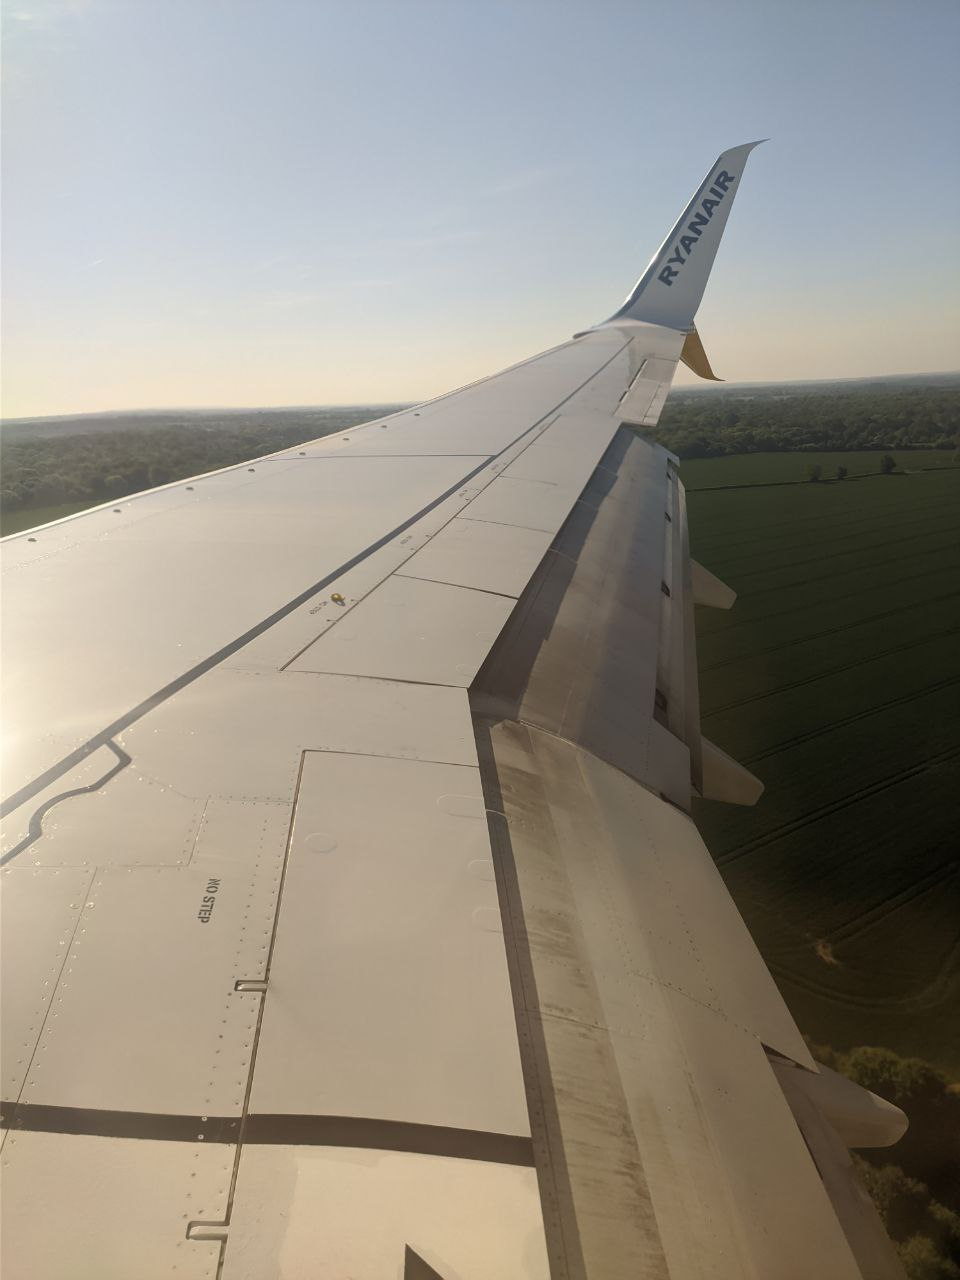
\includegraphics[width=\textwidth]{Images/wing.jpg}
		\end{subfigure}
		\hfill
		\begin{subfigure}{0.45\textwidth}
			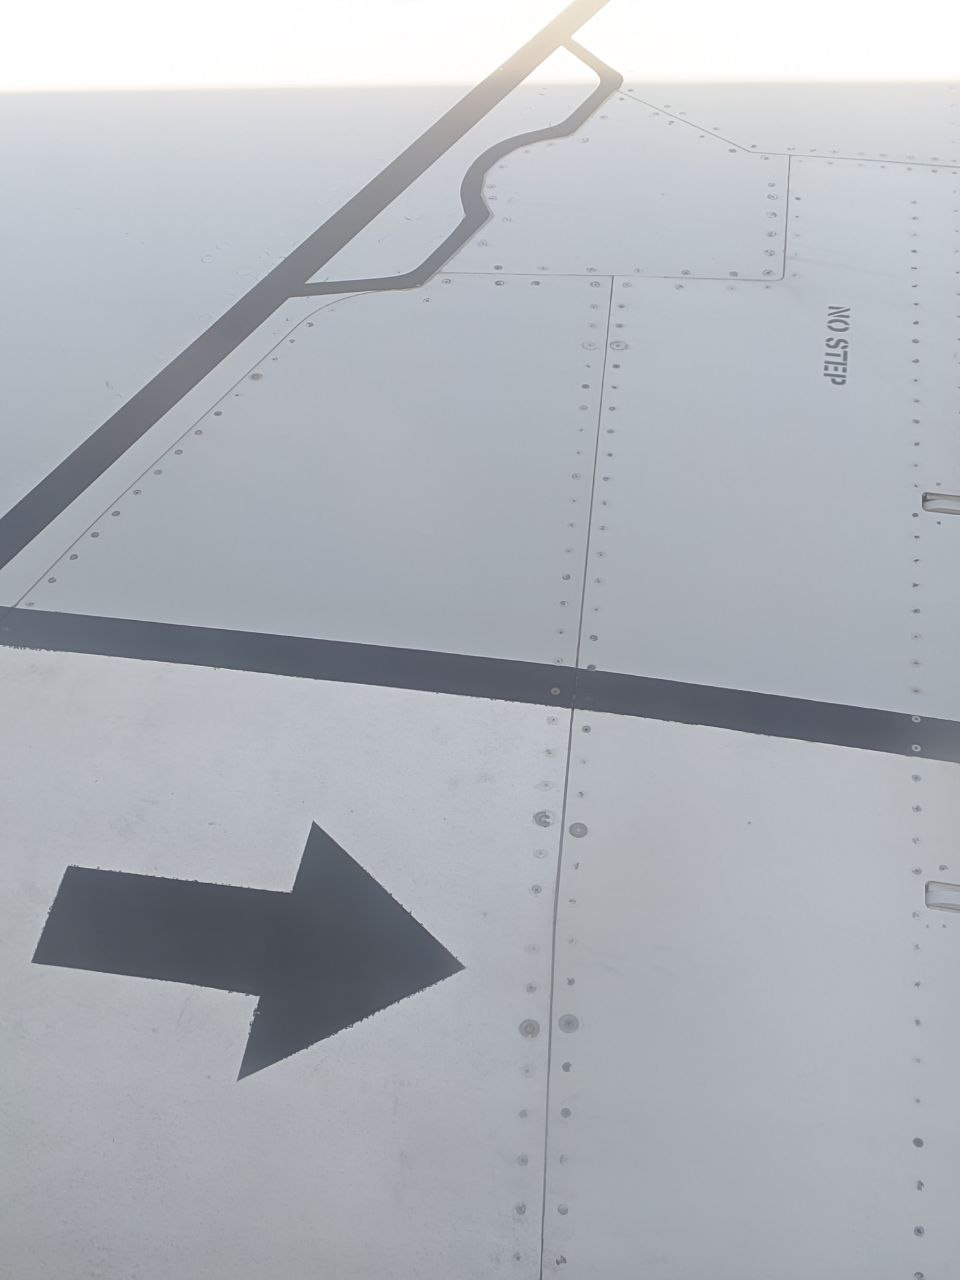
\includegraphics[width=\textwidth]{Images/wing_closer.jpg}
		\end{subfigure}

		\captionof{figure}{Wing of a Boeing 737-800}
	\end{figure}
\end{frame}
\begin{frame}{Setup}

	\begin{figure}[ht]
		\centering
		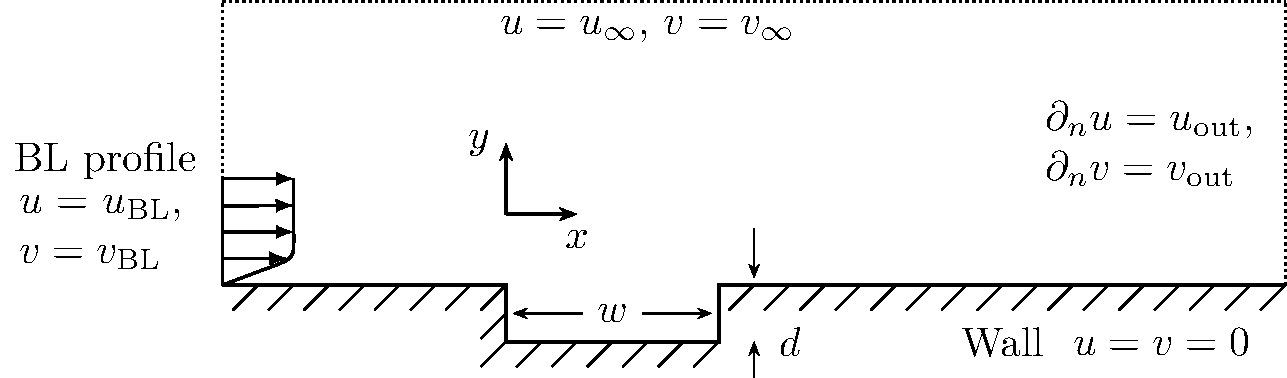
\includegraphics[width=\textwidth]{../../Images/domainBaseflow.pdf}
		\caption{Domain setup for the steady-state finder }
	\end{figure}

	\begin{itemize}
		\item \textbf{Aim:} Study the stability of the system as a function of the depth $d$ and width $w$ of the gap.
		\item 2D incompressible NS
		\item $\text{Re}_{\delta^*} = 1000 \implies\text{Re}_x = 3.38 \times 10^5$
		% \item The reference length is $\delta^*$ measured at the location of the upstream edge of the gap in a surface free of discontinuities (flat plate).
	\end{itemize}

\end{frame}
\begin{frame}{Stability results}
	\begin{figure}
		\begin{flushleft}
			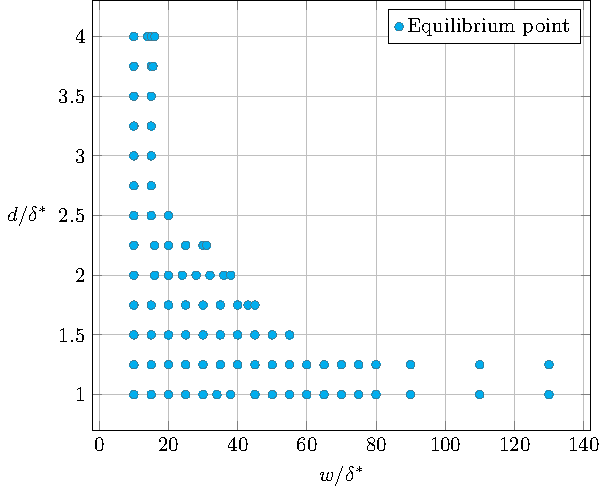
\includegraphics[width=0.5\textwidth]{Images/incNS2dStabilityCurve_equilibria.pdf}
		\end{flushleft}
		\captionof{figure}{\captionstabilityplot}
	\end{figure}
\end{frame}
\begin{frame}{Stability results}
	\begin{figure}
		\centering
		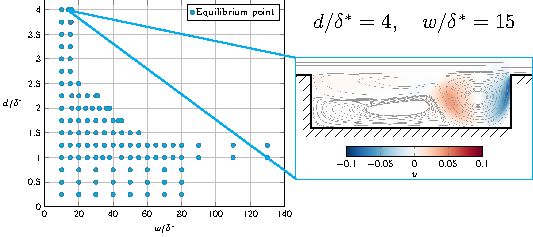
\includegraphics[width=\textwidth]{Images/stablePoints1.pdf}
		\captionof{figure}{\captionstabilityplot}
	\end{figure}
\end{frame}
\begin{frame}{Stability results}
	\begin{figure}
		\centering
		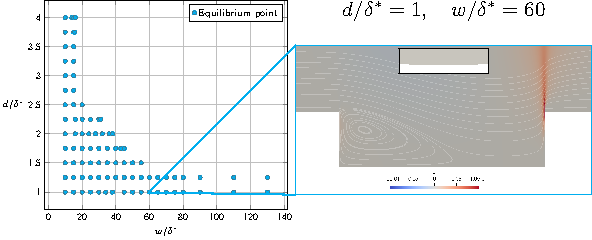
\includegraphics[width=\textwidth]{Images/stablePoints2.pdf}
		\captionof{figure}{\captionstabilityplot}
	\end{figure}
\end{frame}
\begin{frame}{Stability results}
	\begin{figure}
		\begin{flushleft}
			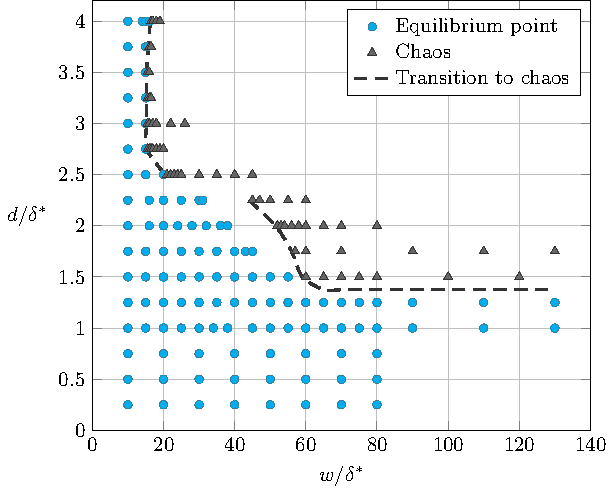
\includegraphics[width=0.5\textwidth]{Images/incNS2dStabilityCurve_partial.pdf}
		\end{flushleft}
		\captionof{figure}{\captionstabilityplot}
	\end{figure}
\end{frame}
\begin{frame}{Stability results}
	\begin{figure}
		\centering
		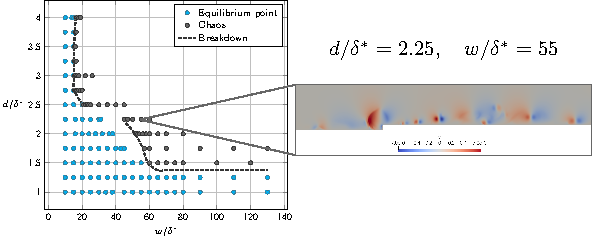
\includegraphics[width=\textwidth]{Images/chaos.pdf}
		\captionof{figure}{\captionstabilityplot}
	\end{figure}
\end{frame}
\begin{frame}{Stability results}
	\begin{figure}
		\begin{flushleft}
			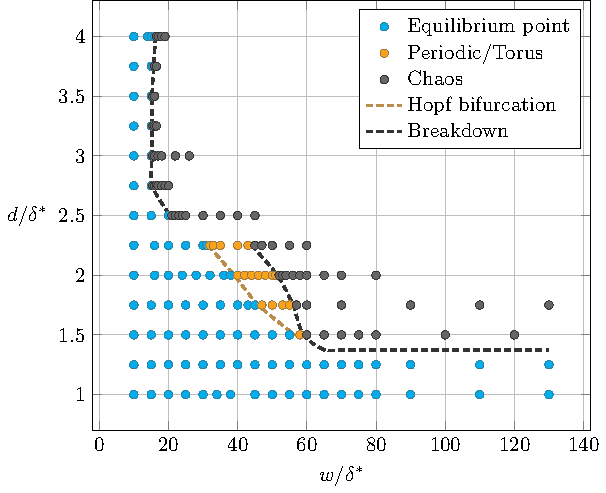
\includegraphics[width=0.5\textwidth]{Images/incNS2dStabilityCurve_full.pdf}
		\end{flushleft}
		\captionof{figure}{\captionstabilityplot}
	\end{figure}
\end{frame}
\begin{frame}{Stability results}
	\begin{figure}
		\centering
		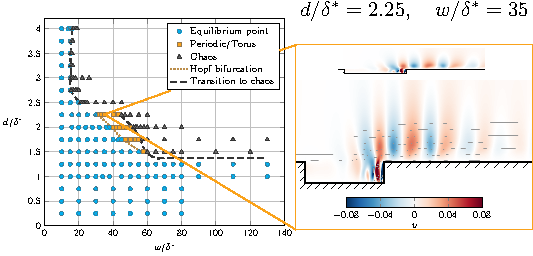
\includegraphics[width=\textwidth]{Images/absUnstable.pdf}
		\captionof{figure}{\captionstabilityplot}
	\end{figure}
\end{frame}
\begin{frame}{Framework for the LST (TS-wave transition)}

	% \begin{itemize}
	% 	\item 2D Incompressible Navier-Stokes\pause
	% 	\item We linearize the flow around a steady baseflow:
	% 	      \onslide<3->{$$\vf{u}(x,y,t) = \vf{U}(x,y)+ \vf{\tilde{u}}(x,y,t)$$}
	% 	\item From LST we can obtain disturbances of the form:
	% 	      \onslide<4->{$$\vf{\tilde{u}} = \vf{\phi}(y) \exp{ -\alpha_i x } \exp{ \ii (\alpha_r x - \omega t) }$$}
	% 	\item But this is a local representation! To account for streamwise growth in the BL we use the $e^N$-method:
	% 	      \onslide<5->{
	% 		      \begin{gather*}
	% 			      n(x, \omega) = -\int_{x_0}^{x} \alpha_i(s,\omega)\dd{s} = \log\left( \frac{\abs{\vf{\tilde{u}}(\omega)}}{\abs{\vf{\tilde{u}}_0}} \right) \\
	% 			      N(x) = \max_{\omega} n(x, \omega)
	% 		      \end{gather*}
	% 		      $\implies$ Disturbances of amplitude $A_0$ satisfy $A(x) \leq A_0 \exp{N(x)}$.}
	% \end{itemize}

	\begin{itemize}
		\item We linearize the flow around a steady baseflow:
		      $$\vf{u}(x,y,t) = \vf{U}(x,y)+ \vf{\tilde{u}}(x,y,t)$$
	\end{itemize}
	\pause
	\begin{itemize}
		\item From LST we can obtain disturbances of the form: $$\vf{\tilde{u}} = \vf{\phi}(y) \exp{ -\alpha_i x } \exp{ \ii (\alpha_r x - \omega t) }$$
	\end{itemize}
	\pause
	\begin{itemize}
		\item But this is a local representation! To account for streamwise growth in the BL we use the $e^N$-method. Fixing $\omega\in \RR$:
		      \begin{gather*}
			      n(x, \omega) = -\int_{x_0}^{x} \alpha_i(s,\omega)\dd{s} = \log\left( \frac{\abs{\vf{\tilde{u}}(x,\omega)}}{\abs{\vf{\tilde{u}}_0}} \right) \\
			      N(x) = \sup_{\omega} n(x, \omega)
		      \end{gather*}
	\end{itemize}\pause
	\begin{itemize}
		$\implies$ Disturbances of amplitude $A_0$ satisfy $A(x) \leq A_0 \exp{N(x)}$.
	\end{itemize}

\end{frame}
\begin{frame}{Previous Work}
	\begin{columns}[T] % [T] ensures correct vertical alignment
		\begin{column}{0.495\linewidth} % Left column
			\vspace{1.5cm}
			\begin{figure}
				\fboxsep=0pt % Remove extra padding inside the frame
				\fbox{
\includegraphics[width=\textwidth]{Images/jeffPaper.pdf}}
			\end{figure}
		\end{column}
		\begin{column}{0.495\linewidth} % Left column
			\begin{figure}
				\vspace{0.15cm}
				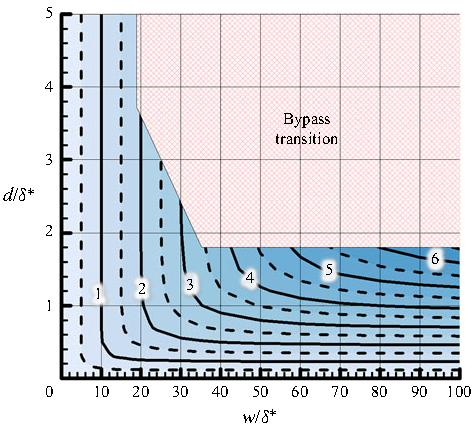
\includegraphics[width=\textwidth]{Images/jeffHeatMap.pdf}
				\captionof{figure}{$\Delta N = N - N_\text{ref}$ for different gap dimensions}
			\end{figure}
		\end{column}
	\end{columns}
	\vspace{0.2cm}

	{\fontsize{6}{8}\selectfont
		\textit{Crouch JD, Kosorygin VS, Sutanto MI, Miller GD. Characterizing surface-gap effects on boundary-layer transition dominated by Tollmien–Schlichting instability. Flow. 2022;2:E8.}}
\end{frame}
\begin{frame}{Perturbed system setup}

	\begin{figure}[ht]
		\centering
		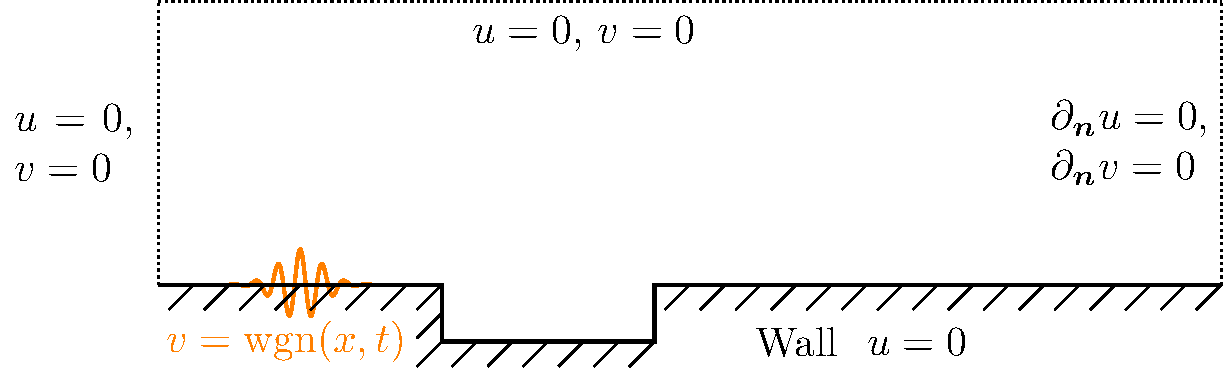
\includegraphics[width=\textwidth]{../../Images/domainPert.pdf}
		\caption{Domain setup for the perturbed system}
	\end{figure}

\end{frame}
\begin{frame}{$\exp{N}$-method results}
	\begin{figure}
		\centering
		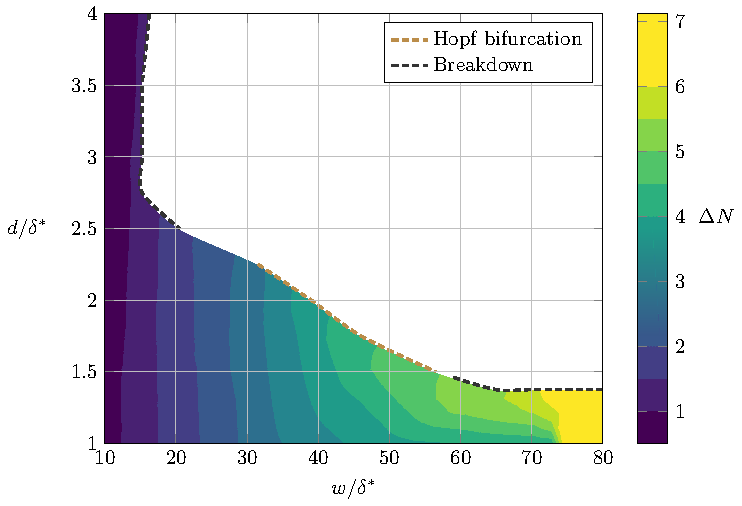
\includegraphics[width=0.8\textwidth]{Images/nfactor_countour_plain.pdf}
		\captionof{figure}{Interpolated $\Delta N = N - N_\text{ref}$ in the globally-stable region.}
	\end{figure}
	\vspace{0.42cm}
\end{frame}
\begin{frame}{$\exp{N}$-method results}
	\begin{figure}
		\centering
		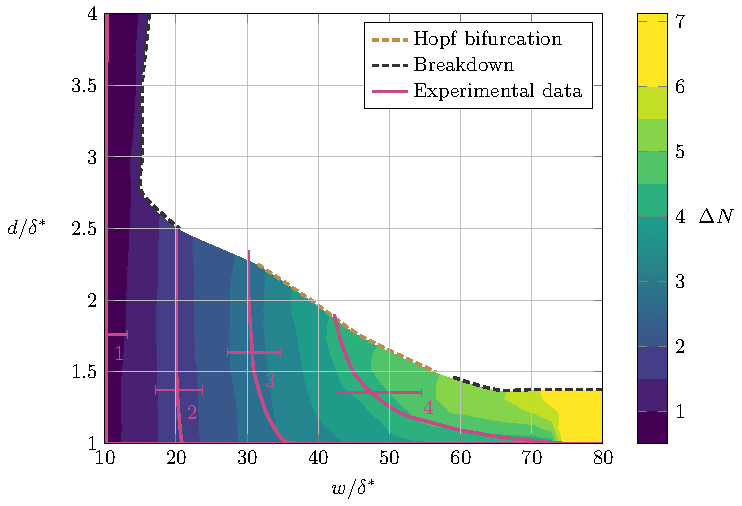
\includegraphics[width=0.8\textwidth]{Images/nfactor_countour.pdf}
		\captionof{figure}{Interpolated $\Delta N = N - N_\text{ref}$ in the equilibra region. Magenta lines indicate the contour levels of the experimental data.}
	\end{figure}
\end{frame}
\begin{frame}{Future Work}
	\begin{itemize}
		\item Go to higher Ma (compressible regime).\pause
		\item Account for spanwise effects (quasi-3d simulations).
	\end{itemize}
\end{frame}
\end{document}
